\documentclass[14pt]{extbook}
\usepackage{multicol, enumerate, enumitem, hyperref, color, soul, setspace, parskip, fancyhdr} %General Packages
\usepackage{amssymb, amsthm, amsmath, latexsym, units, mathtools} %Math Packages
\everymath{\displaystyle} %All math in Display Style
% Packages with additional options
\usepackage[headsep=0.5cm,headheight=12pt, left=1 in,right= 1 in,top= 1 in,bottom= 1 in]{geometry}
\usepackage[usenames,dvipsnames]{xcolor}
\usepackage{dashrule}  % Package to use the command below to create lines between items
\newcommand{\litem}[1]{\item#1\hspace*{-1cm}\rule{\textwidth}{0.4pt}}
\pagestyle{fancy}
\lhead{Progress Quiz 9}
\chead{}
\rhead{Version A}
\lfoot{9541-5764}
\cfoot{}
\rfoot{Summer C 2021}
\begin{document}

\begin{enumerate}
\litem{
First, find the equation of the line containing the two points below. Then, write the equation in the form $ y=mx+b $ and choose the intervals that contain $m$ and $b$.\[ (4, -10) \text{ and } (-10, 4) \]\begin{enumerate}[label=\Alph*.]
\item \( m \in [-3.2, -0.3] \hspace*{3mm} b \in [4, 12] \)
\item \( m \in [-3.2, -0.3] \hspace*{3mm} b \in [-12, -3] \)
\item \( m \in [0.8, 1.1] \hspace*{3mm} b \in [10, 18] \)
\item \( m \in [-3.2, -0.3] \hspace*{3mm} b \in [10, 18] \)
\item \( m \in [-3.2, -0.3] \hspace*{3mm} b \in [-15, -11] \)

\end{enumerate} }
\litem{
Solve the equation below. Then, choose the interval that contains the solution.\[ -16(-11x + 2) = -5(17x -18) \]\begin{enumerate}[label=\Alph*.]
\item \( x \in [-0.38, -0.21] \)
\item \( x \in [0.46, 0.71] \)
\item \( x \in [-1.16, -0.56] \)
\item \( x \in [-0.07, 0.29] \)
\item \( \text{There are no real solutions.} \)

\end{enumerate} }
\litem{
Solve the equation below. Then, choose the interval that contains the solution.\[ -9(3x -19) = -12(7x -18) \]\begin{enumerate}[label=\Alph*.]
\item \( x \in [0.4, 0.9] \)
\item \( x \in [4.7, 7] \)
\item \( x \in [-8.5, -6.5] \)
\item \( x \in [2.8, 3.8] \)
\item \( \text{There are no real solutions.} \)

\end{enumerate} }
\litem{
First, find the equation of the line containing the two points below. Then, write the equation in the form $ y=mx+b $ and choose the intervals that contain $m$ and $b$.\[ (-8, 11) \text{ and } (-3, -8) \]\begin{enumerate}[label=\Alph*.]
\item \( m \in [3.8, 4.8] \hspace*{3mm} b \in [3.27, 3.59] \)
\item \( m \in [-11.8, -1.8] \hspace*{3mm} b \in [19.25, 19.6] \)
\item \( m \in [-11.8, -1.8] \hspace*{3mm} b \in [-5.52, -4.94] \)
\item \( m \in [-11.8, -1.8] \hspace*{3mm} b \in [18.55, 19.3] \)
\item \( m \in [-11.8, -1.8] \hspace*{3mm} b \in [-19.71, -19.2] \)

\end{enumerate} }
\litem{
Find the equation of the line described below. Write the linear equation in the form $ y=mx+b $ and choose the intervals that contain $m$ and $b$.\[ \text{Perpendicular to } 8 x + 7 y = 6 \text{ and passing through the point } (4, 5). \]\begin{enumerate}[label=\Alph*.]
\item \( m \in [0.83, 1] \hspace*{3mm} b \in [1.41, 2.39] \)
\item \( m \in [-0.9, -0.74] \hspace*{3mm} b \in [8.16, 8.58] \)
\item \( m \in [0.83, 1] \hspace*{3mm} b \in [-1.77, -1.45] \)
\item \( m \in [0.83, 1] \hspace*{3mm} b \in [0.58, 1.29] \)
\item \( m \in [0.98, 1.25] \hspace*{3mm} b \in [1.41, 2.39] \)

\end{enumerate} }
\litem{
Write the equation of the line in the graph below in Standard Form $Ax+By=C$. Then, choose the intervals that contain $A, B, \text{ and } C$.
\begin{center}
    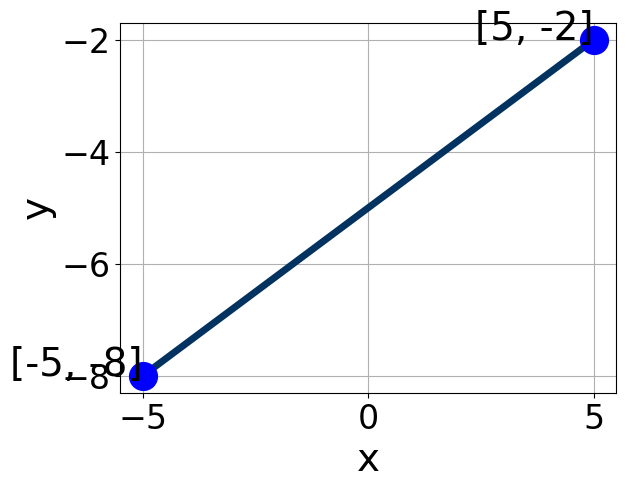
\includegraphics[width=0.5\textwidth]{../Figures/linearGraphToStandardA.png}
\end{center}
\begin{enumerate}[label=\Alph*.]
\item \( A \in [-2.7, 1.1], \hspace{3mm} B \in [-4.6, 0.3], \text{ and } \hspace{3mm} C \in [1, 7] \)
\item \( A \in [2.5, 5], \hspace{3mm} B \in [3.8, 5.1], \text{ and } \hspace{3mm} C \in [-31, -22] \)
\item \( A \in [2.5, 5], \hspace{3mm} B \in [-6, -1.5], \text{ and } \hspace{3mm} C \in [23, 28] \)
\item \( A \in [-4.8, -2.7], \hspace{3mm} B \in [3.8, 5.1], \text{ and } \hspace{3mm} C \in [-31, -22] \)
\item \( A \in [-2.7, 1.1], \hspace{3mm} B \in [0.9, 2.6], \text{ and } \hspace{3mm} C \in [-7, -4] \)

\end{enumerate} }
\litem{
Solve the linear equation below. Then, choose the interval that contains the solution.\[ \frac{3x + 6}{8} - \frac{-3x -8}{5} = \frac{9x + 5}{7} \]\begin{enumerate}[label=\Alph*.]
\item \( x \in [27.97, 30.97] \)
\item \( x \in [5.26, 6.26] \)
\item \( x \in [-0.45, 1.55] \)
\item \( x \in [-8.03, -4.03] \)
\item \( \text{There are no real solutions.} \)

\end{enumerate} }
\litem{
Solve the linear equation below. Then, choose the interval that contains the solution.\[ \frac{4x + 9}{3} - \frac{-9x + 3}{7} = \frac{5x -4}{2} \]\begin{enumerate}[label=\Alph*.]
\item \( x \in [-5.57, 0.43] \)
\item \( x \in [-84, -80] \)
\item \( x \in [-41.4, -36.4] \)
\item \( x \in [-45.6, -43.6] \)
\item \( \text{There are no real solutions.} \)

\end{enumerate} }
\litem{
Write the equation of the line in the graph below in Standard Form $Ax+By=C$. Then, choose the intervals that contain $A, B, \text{ and } C$.
\begin{center}
    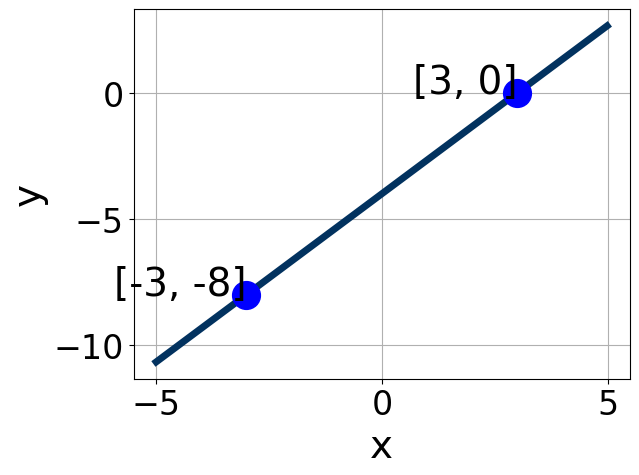
\includegraphics[width=0.5\textwidth]{../Figures/linearGraphToStandardCopyA.png}
\end{center}
\begin{enumerate}[label=\Alph*.]
\item \( A \in [-2.2, 0.8], \hspace{3mm} B \in [-0.09, 1.58], \text{ and } \hspace{3mm} C \in [-7, -3] \)
\item \( A \in [-4.6, -2.6], \hspace{3mm} B \in [1.71, 3.62], \text{ and } \hspace{3mm} C \in [-13, -10] \)
\item \( A \in [1.9, 4.6], \hspace{3mm} B \in [-3.18, -2.15], \text{ and } \hspace{3mm} C \in [12, 16] \)
\item \( A \in [-2.2, 0.8], \hspace{3mm} B \in [-1.34, -0.92], \text{ and } \hspace{3mm} C \in [0, 9] \)
\item \( A \in [1.9, 4.6], \hspace{3mm} B \in [1.71, 3.62], \text{ and } \hspace{3mm} C \in [-13, -10] \)

\end{enumerate} }
\litem{
Find the equation of the line described below. Write the linear equation in the form $ y=mx+b $ and choose the intervals that contain $m$ and $b$.\[ \text{Perpendicular to } 3 x + 8 y = 4 \text{ and passing through the point } (4, -10). \]\begin{enumerate}[label=\Alph*.]
\item \( m \in [2.5, 4.8] \hspace*{3mm} b \in [-16, -9] \)
\item \( m \in [2.5, 4.8] \hspace*{3mm} b \in [-23.67, -19.67] \)
\item \( m \in [-0.5, 2.6] \hspace*{3mm} b \in [-23.67, -19.67] \)
\item \( m \in [2.5, 4.8] \hspace*{3mm} b \in [17.67, 22.67] \)
\item \( m \in [-5.3, -1.6] \hspace*{3mm} b \in [-1.33, 3.67] \)

\end{enumerate} }
\end{enumerate}

\end{document}